% !TeX TXS-program:compile = txs:///knit2pdf
\documentclass[12pt]{mwart}\usepackage[]{graphicx}\usepackage[]{color}
% maxwidth is the original width if it is less than linewidth
% otherwise use linewidth (to make sure the graphics do not exceed the margin)
\makeatletter
\def\maxwidth{ %
  \ifdim\Gin@nat@width>\linewidth
    \linewidth
  \else
    \Gin@nat@width
  \fi
}
\makeatother

\definecolor{fgcolor}{rgb}{0.345, 0.345, 0.345}
\newcommand{\hlnum}[1]{\textcolor[rgb]{0.686,0.059,0.569}{#1}}%
\newcommand{\hlstr}[1]{\textcolor[rgb]{0.192,0.494,0.8}{#1}}%
\newcommand{\hlcom}[1]{\textcolor[rgb]{0.678,0.584,0.686}{\textit{#1}}}%
\newcommand{\hlopt}[1]{\textcolor[rgb]{0,0,0}{#1}}%
\newcommand{\hlstd}[1]{\textcolor[rgb]{0.345,0.345,0.345}{#1}}%
\newcommand{\hlkwa}[1]{\textcolor[rgb]{0.161,0.373,0.58}{\textbf{#1}}}%
\newcommand{\hlkwb}[1]{\textcolor[rgb]{0.69,0.353,0.396}{#1}}%
\newcommand{\hlkwc}[1]{\textcolor[rgb]{0.333,0.667,0.333}{#1}}%
\newcommand{\hlkwd}[1]{\textcolor[rgb]{0.737,0.353,0.396}{\textbf{#1}}}%
\let\hlipl\hlkwb

\usepackage{framed}
\makeatletter
\newenvironment{kframe}{%
 \def\at@end@of@kframe{}%
 \ifinner\ifhmode%
  \def\at@end@of@kframe{\end{minipage}}%
  \begin{minipage}{\columnwidth}%
 \fi\fi%
 \def\FrameCommand##1{\hskip\@totalleftmargin \hskip-\fboxsep
 \colorbox{shadecolor}{##1}\hskip-\fboxsep
     % There is no \\@totalrightmargin, so:
     \hskip-\linewidth \hskip-\@totalleftmargin \hskip\columnwidth}%
 \MakeFramed {\advance\hsize-\width
   \@totalleftmargin\z@ \linewidth\hsize
   \@setminipage}}%
 {\par\unskip\endMakeFramed%
 \at@end@of@kframe}
\makeatother

\definecolor{shadecolor}{rgb}{.97, .97, .97}
\definecolor{messagecolor}{rgb}{0, 0, 0}
\definecolor{warningcolor}{rgb}{1, 0, 1}
\definecolor{errorcolor}{rgb}{1, 0, 0}
\newenvironment{knitrout}{}{} % an empty environment to be redefined in TeX

\usepackage{alltt}
\usepackage[utf8]{inputenc}
\usepackage[T1,plmath]{polski}
\usepackage{lmodern}

\usepackage{amssymb}
\usepackage{graphicx}
\usepackage{amsmath}
\usepackage{amsthm}
\usepackage[hidelinks]{hyperref}
\usepackage{float}

\title{Sprawozdanie 1}
\author{Aleksander Jakóbczyk i Kacper Pasterniak}
\date{}
\IfFileExists{upquote.sty}{\usepackage{upquote}}{}
\begin{document}
	\maketitle 
	

	
	\section*{Lista 1}
  \subsection*{Zad 1}
  \subsubsection*{Detergent}
\begin{knitrout}\small
\definecolor{shadecolor}{rgb}{0.969, 0.969, 0.969}\color{fgcolor}\begin{kframe}
\begin{alltt}
\hlstd{Detergent.df} \hlkwb{<-} \hlkwd{data.frame}\hlstd{(Detergent)}
\hlstd{Detergent.df} \hlopt \hlkwd{group_by}\hlstd{(Temperature)} \hlopt \hlkwd{summarise}\hlstd{(}\hlkwc{n} \hlstd{=} \hlkwd{sum}\hlstd{(Freq))}
\end{alltt}
\begin{verbatim}
## # A tibble: 2 x 2
##   Temperature     n
##   <fct>       <dbl>
## 1 High          369
## 2 Low           639
\end{verbatim}
\begin{alltt}
\hlstd{Detergent.df} \hlopt \hlkwd{filter}\hlstd{(Water_softness} \hlopt{==} \hlstr{"Soft"}\hlstd{)} \hlopt \hlkwd{group_by}\hlstd{(Temperature)} \hlopt \hlkwd{summarise}\hlstd{(}\hlkwc{n} \hlstd{=} \hlkwd{sum}\hlstd{(Freq))}
\end{alltt}
\begin{verbatim}
## # A tibble: 2 x 2
##   Temperature     n
##   <fct>       <dbl>
## 1 High          104
## 2 Low           222
\end{verbatim}
\begin{alltt}
\hlstd{Detergent.df} \hlopt \hlkwd{filter}\hlstd{(Water_softness} \hlopt{==} \hlstr{"Medium"}\hlstd{)} \hlopt \hlkwd{group_by}\hlstd{(Temperature)} \hlopt \hlkwd{summarise}\hlstd{(}\hlkwc{n} \hlstd{=} \hlkwd{sum}\hlstd{(Freq))}
\end{alltt}
\begin{verbatim}
## # A tibble: 2 x 2
##   Temperature     n
##   <fct>       <dbl>
## 1 High          126
## 2 Low           218
\end{verbatim}
\begin{alltt}
\hlstd{Detergent.df} \hlopt \hlkwd{filter}\hlstd{(Water_softness} \hlopt{==} \hlstr{"Hard"}\hlstd{)} \hlopt \hlkwd{group_by}\hlstd{(Temperature)} \hlopt \hlkwd{summarise}\hlstd{(}\hlkwc{n} \hlstd{=} \hlkwd{sum}\hlstd{(Freq))}
\end{alltt}
\begin{verbatim}
## # A tibble: 2 x 2
##   Temperature     n
##   <fct>       <dbl>
## 1 High          139
## 2 Low           199
\end{verbatim}
\end{kframe}
\end{knitrout}

  \subsubsection*{Preference}

\begin{knitrout}\small
\definecolor{shadecolor}{rgb}{0.969, 0.969, 0.969}\color{fgcolor}\begin{kframe}
\begin{alltt}
\hlcom{# Detergent.df %>% group_by(Preference) %>% summarise(n = sum(Freq))}
\hlstd{Detergent.df} \hlopt \hlkwd{filter}\hlstd{(Water_softness} \hlopt{==} \hlstr{"Soft"}\hlstd{)} \hlopt \hlkwd{group_by}\hlstd{(Preference)} \hlopt \hlkwd{summarise}\hlstd{(}\hlkwc{n} \hlstd{=} \hlkwd{sum}\hlstd{(Freq))}
\end{alltt}
\begin{verbatim}
## # A tibble: 2 x 2
##   Preference     n
##   <fct>      <dbl>
## 1 Brand X      168
## 2 Brand M      158
\end{verbatim}
\begin{alltt}
\hlstd{Detergent.df} \hlopt \hlkwd{filter}\hlstd{(Water_softness} \hlopt{==} \hlstr{"Medium"}\hlstd{)} \hlopt \hlkwd{group_by}\hlstd{(Preference)} \hlopt \hlkwd{summarise}\hlstd{(}\hlkwc{n} \hlstd{=} \hlkwd{sum}\hlstd{(Freq))}
\end{alltt}
\begin{verbatim}
## # A tibble: 2 x 2
##   Preference     n
##   <fct>      <dbl>
## 1 Brand X      169
## 2 Brand M      175
\end{verbatim}
\begin{alltt}
\hlstd{Detergent.df} \hlopt \hlkwd{filter}\hlstd{(Water_softness} \hlopt{==} \hlstr{"Hard"}\hlstd{)} \hlopt \hlkwd{group_by}\hlstd{(Preference)} \hlopt \hlkwd{summarise}\hlstd{(}\hlkwc{n} \hlstd{=} \hlkwd{sum}\hlstd{(Freq))}
\end{alltt}
\begin{verbatim}
## # A tibble: 2 x 2
##   Preference     n
##   <fct>      <dbl>
## 1 Brand X      171
## 2 Brand M      167
\end{verbatim}
\end{kframe}
\end{knitrout}

  \subsection*{Zad 2}
\begin{knitrout}
\definecolor{shadecolor}{rgb}{0.969, 0.969, 0.969}\color{fgcolor}\begin{kframe}
\begin{alltt}
\hlkwd{ftable}\hlstd{(Detergent,} \hlkwc{col.vars} \hlstd{=} \hlstr{"Temperature"}\hlstd{,} \hlkwc{row.vars} \hlstd{=} \hlstr{"Water_softness"}\hlstd{)}
\end{alltt}
\begin{verbatim}
##                Temperature High Low
## Water_softness                     
## Soft                        104 222
## Medium                      126 218
## Hard                        139 199
\end{verbatim}
\begin{alltt}
\hlkwd{structable}\hlstd{(Temperature} \hlopt{~} \hlstd{Water_softness, Detergent)} \hlopt \hlkwd{addmargins}\hlstd{()}
\end{alltt}
\begin{verbatim}
##               Temperature
## Water_softness High Low  Sum
##         Soft    104 222  326
##         Medium  126 218  344
##         Hard    139 199  338
##         Sum     369 639 1008
\end{verbatim}
\end{kframe}
\end{knitrout}

  \subsection*{Zad 3}
\begin{knitrout}
\definecolor{shadecolor}{rgb}{0.969, 0.969, 0.969}\color{fgcolor}\begin{kframe}
\begin{alltt}
\hlstd{A} \hlkwb{<-} \hlkwd{apply}\hlstd{(Detergent,} \hlstr{"Water_softness"}\hlstd{, sum)}
\hlkwd{barplot}\hlstd{(A)}
\end{alltt}
\end{kframe}\begin{figure}[H]
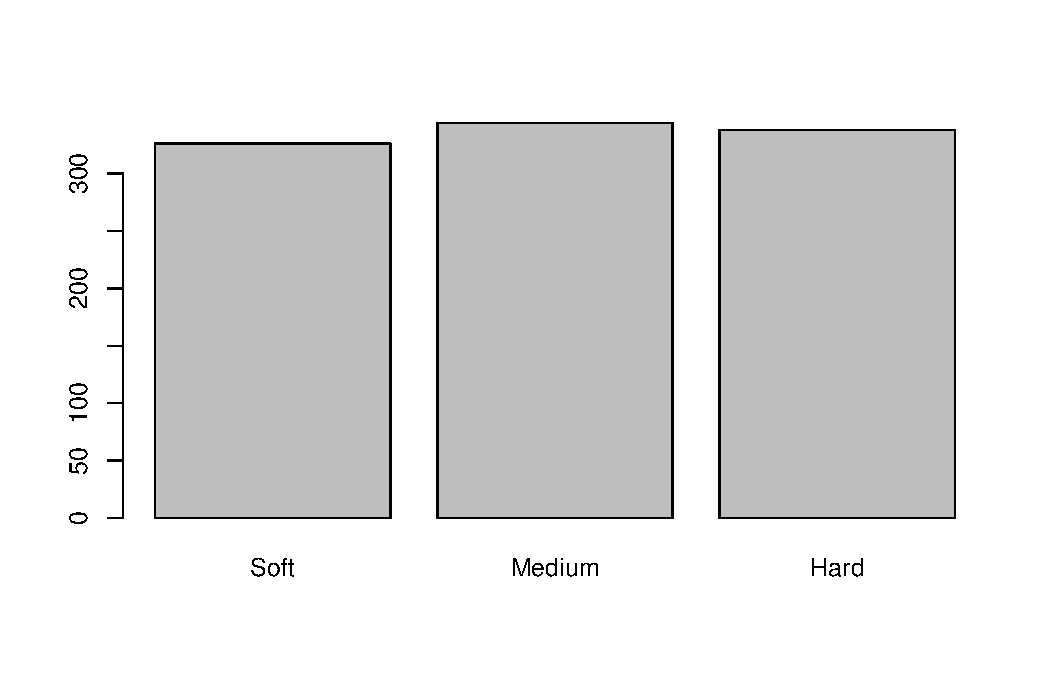
\includegraphics[width=\maxwidth]{figure/r_fig_1-1} \caption{\label{fig:1}Wykresy słupkowy dla mniennej Water Softness.}\label{fig:r fig_1}
\end{figure}

\end{knitrout}
\begin{knitrout}
\definecolor{shadecolor}{rgb}{0.969, 0.969, 0.969}\color{fgcolor}\begin{kframe}
\begin{alltt}
\hlkwd{par}\hlstd{(}\hlkwc{mar} \hlstd{=} \hlkwd{c}\hlstd{(}\hlnum{2}\hlstd{,} \hlnum{2}\hlstd{,} \hlnum{2}\hlstd{,} \hlnum{2}\hlstd{))}
\hlkwd{pie}\hlstd{(A)}
\end{alltt}
\end{kframe}\begin{figure}[H]
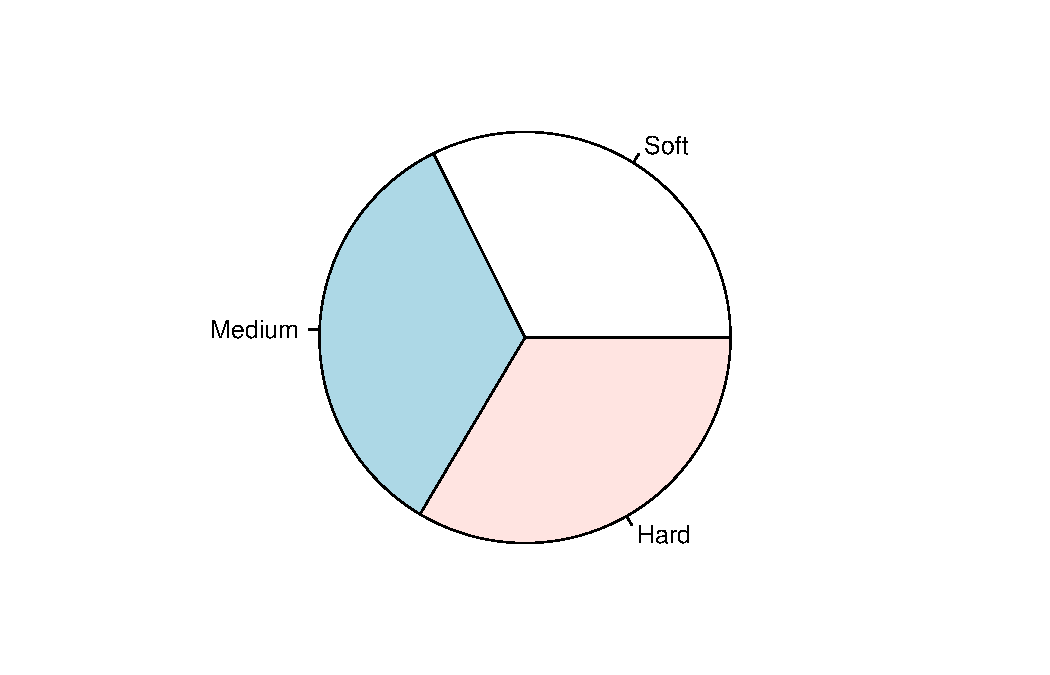
\includegraphics[width=\maxwidth]{figure/r_fig_2-1} \caption{\label{fig:2}Wykresy kołowy dla mniennej Water Softness.}\label{fig:r fig_2}
\end{figure}

\end{knitrout}
  \subsection*{Zad 4}
\begin{knitrout}
\definecolor{shadecolor}{rgb}{0.969, 0.969, 0.969}\color{fgcolor}\begin{kframe}
\begin{alltt}
\hlkwd{par}\hlstd{(}\hlkwc{mar} \hlstd{=} \hlkwd{c}\hlstd{(}\hlnum{2}\hlstd{,} \hlnum{2}\hlstd{,} \hlnum{2}\hlstd{,} \hlnum{2}\hlstd{))}
\hlkwd{mosaicplot}\hlstd{(}\hlopt{~}\hlstd{Water_softness}\hlopt{+}\hlstd{Preference,} \hlkwc{data} \hlstd{= Detergent)}
\end{alltt}
\end{kframe}\begin{figure}[H]
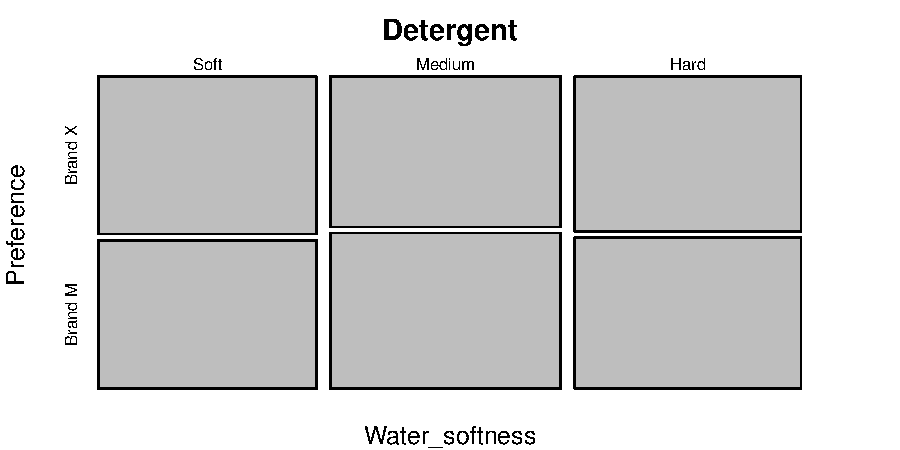
\includegraphics[width=\maxwidth]{figure/r_fig_3-1} \caption{\label{fig:3}Wykres mozajkowy dla Preference i Water softness}\label{fig:r fig_3}
\end{figure}

\end{knitrout}
\begin{knitrout}
\definecolor{shadecolor}{rgb}{0.969, 0.969, 0.969}\color{fgcolor}\begin{kframe}
\begin{alltt}
\hlkwd{par}\hlstd{(}\hlkwc{mar} \hlstd{=} \hlkwd{c}\hlstd{(}\hlnum{2}\hlstd{,} \hlnum{2}\hlstd{,} \hlnum{2}\hlstd{,} \hlnum{2}\hlstd{))}
\hlkwd{mosaicplot}\hlstd{(}\hlopt{~}\hlstd{M_User}\hlopt{+}\hlstd{Preference,} \hlkwc{data} \hlstd{= Detergent)}
\end{alltt}
\end{kframe}\begin{figure}[H]
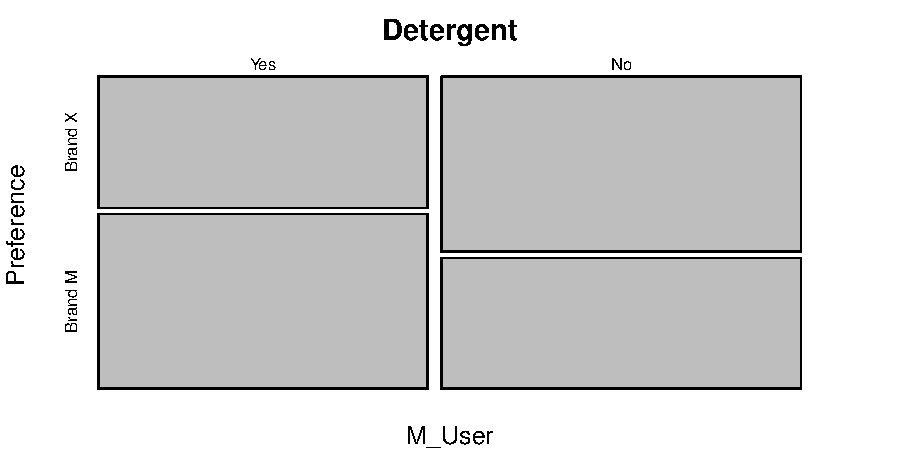
\includegraphics[width=\maxwidth]{figure/r_fig_4-1} \caption{\label{fig:4}Wykres mozajkowy dla Preference i M User.}\label{fig:r fig_4}
\end{figure}

\end{knitrout}
\begin{knitrout}
\definecolor{shadecolor}{rgb}{0.969, 0.969, 0.969}\color{fgcolor}\begin{kframe}
\begin{alltt}
\hlkwd{par}\hlstd{(}\hlkwc{mar} \hlstd{=} \hlkwd{c}\hlstd{(}\hlnum{2}\hlstd{,} \hlnum{2}\hlstd{,} \hlnum{2}\hlstd{,} \hlnum{2}\hlstd{))}
\hlkwd{mosaicplot}\hlstd{(}\hlopt{~}\hlstd{Temperature}\hlopt{+}\hlstd{Preference,} \hlkwc{data} \hlstd{= Detergent)}
\end{alltt}
\end{kframe}\begin{figure}[H]
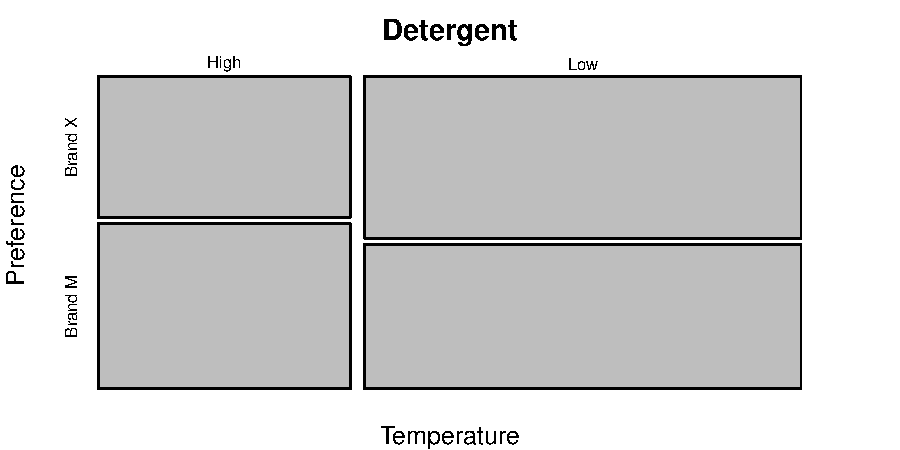
\includegraphics[width=\maxwidth]{figure/r_fig_5-1} \caption{\label{fig:5}Wykres mozajkowy dla Preference i Temperature.}\label{fig:r fig_5}
\end{figure}

\end{knitrout}
\end{document}
